\chapter{Virtual cortical resection reveals push-pull network control mechanism}
\label{ch:selfreg}

% the code below specifies where the figures are stored
\ifpdf
    \graphicspath{{chapters/ch5_figures/PNG/}{chapters/ch5_figures/PDF/}{chapters/ch5_figures/}}
\else
    \graphicspath{{chapters/ch5_figures/EPS/}{chapters/ch5_figures/}}
\fi


% ----------------------------------------------------------------------
%: ----------------------- content ----------------------- 
% ----------------------------------------------------------------------
\section{Abstract}
For $\approx$20 million people with drug-resistant epilepsy, recurring, spontaneous seizures have devastating impact on daily life. Current treatment options for these patients are resective surgery, and more recently, implantable devices to control seizures. The efficacy of these therapies is hindered by a poor understanding of why some seizures spread to surrounding tissue while others remain focal and confined. Network mechanisms that regulate synchronization between connected brain regions may explain differential seizure dynamics. To pinpoint network regions that regulate seizure evolution, we present a novel method to assess changes in synchronizability in response to virtually lesioning cortical areas in a validated computational network model. We apply our virtual cortical resection technique to time-varying functional networks measured in 10 human patients implanted with electrocorticographic sensors for clinical localization of their epilepsy. Our results suggest that the network's synchronizability prior to seizure onset predicts the extent of seizure evolution. Using virtual cortical resection, i.e. selectively removing nodes from the computational model, we identify important control regions that drive network behavior by individually desynchronizing or synchronizing distinct cortical areas. We find that for seizures that remain focal, the strongest controllers preceding seizures are localized outside seizure-generating areas. Our results support the notion that these controllers utilize an antagonistic push-pull control scheme to regulate network synchronizability. These studies suggest that tailoring therapy to leverage regulatory mechanisms that constrain the extent of seizure spread may improve existing treatment. 

\section{Introduction}
Functional architecture of the epileptic neocortex has been studied extensively to better identify optimal targets for surgical resection and, more recently, the optimal location for implantable devices. The prospect of patient-centric algorithms that modulate brain state to abort seizures is exciting to clinicians and researchers alike \cite{morrell2011responsive, stanslaski2012design, afshar2013translational}. However, the best targets for chronic devices remain elusive, partly because functional brain networks, including epileptic networks, reorganize dynamically \cite{bassett2006adaptive, bassett2011dynamic, rummel2013systems-level, burns2014network}. Such reorganization appear to follow a specific progression through network states unique to the patient's seizures \cite{wulsin2013parsing, burns2014network}. The mechanisms that drive seizures through network states can inform neural control paradigms that aim to stop or contain propagation of seizure activity. Such a capability is vital, clinically, because epileptogenic regions cause symptoms not only through their own dysfunction, but also through their ability to recruit and disrupt normal brain regions \cite{kutsy1999ictal}. However, understanding and translating network mechanisms of seizure evolution to identify targets for therapy requires further dissection of functional epileptic network architecture. 

Conventional school of thought divides epileptic brain into the \textit{seizure-onset} or \textit{ictal zone}, a clinically-defined where seizures are generated, and the \textit{irritative zone}, which emits non-seizure-generating epileptiform events including spike-wave discharges and high-frequency oscillations \cite{rosenow2001presurgical}. Recent models describe connectivity between the seizure-onset and irritative zones in the framework of a broader dysfunctional \textit{epileptic network}, where network nodes are neural populations measured by intracranial sensors and network connections are statistical relationships between neural activation patterns \cite{nair2004critical, kramer2010coalescence, warren2010synchrony, wilke2011graph, burns2014network} (\textbf{Fig.~\ref{ch5:fig1}A}). For example, partial seizures that begin in the seizure-onset zone can evolve, spreading spatially as they modulate in dominant frequency, via local connections to the surrounding tissue, implicating a distributed epileptic network \cite{spencer2002neural, nair2004critical, kramer2010coalescence, korzeniewska2014ictal}. In the extreme case these seizures secondarily generalize to encompass the entire brain.

Given the distributed nature of epileptic activity, it is critical to isolate underlying propagation mechanisms. Leading hypotheses suggest that either (i) seizure evolution is driven by strong, synchronizing activity from the seizure-generating network impinging outward on the surrounding tissue \cite{schindler2008evolving, kramer2010coalescence, kramer2012epilepsy, jiruska2012synchronization}, or (ii) seizure evolution is caused by a diminished ability of the surrounding tissue to regulate, or contain, abnormal activity \cite{nair2004critical, bower2012spatiotemporal}. While little evidence exists to determine which of these hypotheses accurately reflect seizure dynamics, both mechanisms can be succinctly summarized as abnormalities of synchronizability, a description of how easily neural processes, such as rhythmic activity, can flow through a network.

Theoretical work demonstrates that the synchronizability of a system can be regulated through a \textit{push-pull control} mechanism, where desynchronizing and synchronizing nodes operate antagonistically in a ``tug-of-war'' to maintain network stability. When desynchronizing, synchronizing or both forces weaken, network stability is compromised such that the network is driven to a different state \cite{he2014control} (\textbf{Fig.~\ref{ch5:fig1}B}). Such mechanisms are particularly successful in heterogeneous networks like the brain, where some nodes are sparsely connected and other nodes are densely connected \cite{wang2002synchronization}. Does the brain utilize such a control mechanism for seizure regulation? And if so, what regions of the brain affect this control?

To address these questions, we present a novel method we call \textit{virtual cortical resection}, which offers a statistically robust means to pinpoint putative control nodes in the epileptic network that may regulate seizure dynamics, based on the network's response to virtual lesioning \cite{wang2002synchronization, wang2002pinning}. We use this method to test the hypothesis that the epileptic network contains a native regulatory system (\textbf{Fig.~\ref{ch5:fig1}C}) whose connectivity to the seizure-generating area accounts for differential seizure dynamics, including (i) the constrained dynamics observed in partial seizures that remain focal (\textbf{Fig.~\ref{ch5:fig1}D}), and (ii) the unconstrained dynamics observed in partial seizures that generalize to surrounding tissue (\textbf{Fig.~\ref{ch5:fig1}E}).

More specifically, using electrocorticography recorded from 10 patients diagnosed with drug-resistant neocortical epilepsy undergoing routine pre-surgical evaluation, we constructed time-evolving functional networks across \emph{events}, each of which included a seizure epoch preceded by a pre-seizure epoch. The seizure epoch spanned the period between the clinically-marked earliest electrographic change \cite{litt2001epileptic} and the seizure termination, while the pre-seizure epoch was identical in duration to the seizure and ended immediately prior to the earliest electrographic change. In each epoch we divided the ECoG signal into 1s non-overlapping time-windows and estimated functional connectivity in a high-$\gamma$ (95--105 Hz) frequency band using multitaper coherence estimation (see \textit{Methods}). We implemented virtual cortical resection on this dynamic epileptic network by independently removing electrode sites from the network model. This was done to assess the synchronizability of (i) the distributed epileptic network in partial seizures that generalize to surrounding tissue, \emph{versus} (ii) the focal epileptic network in those that do not. By removing electrode sites from the network model, we were able to probe the importance brain regions, in their presence and absence, to seizure generation and propagation.

\begin{figure}[H]
    \centering
    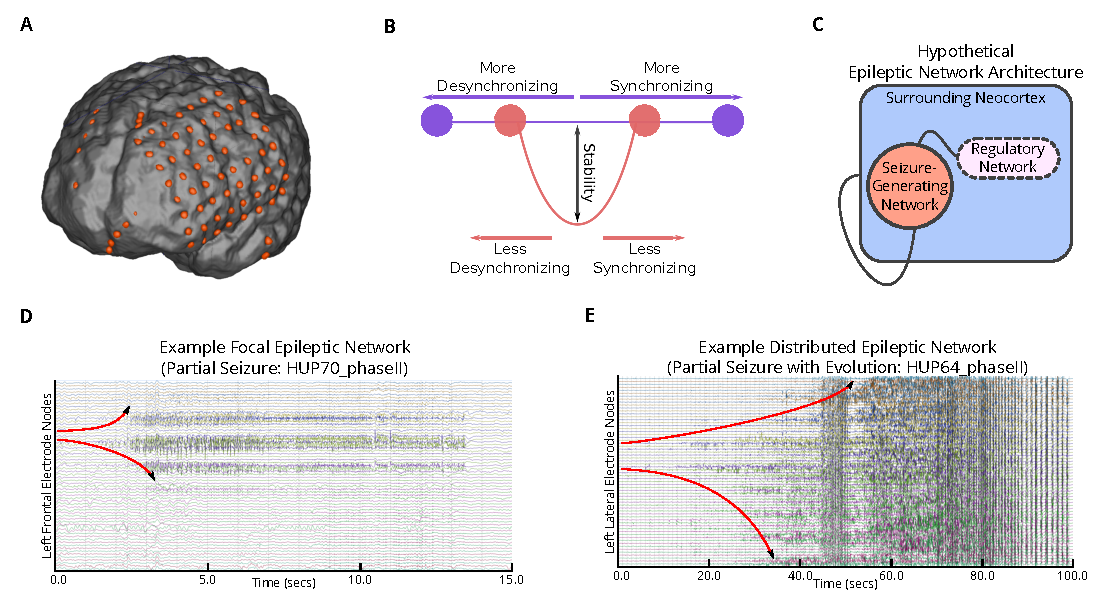
\includegraphics[width=\textwidth]{panel1.eps}
    \caption[Hypothetical regulatory mechansim of seizure spread]{\textbf{Hypothesized regulatory mechanism of seizure spread} (\textbf{A}) We create functional networks based on electrophysiology from patients with drug-resistant neocortical epilepsy implanted with intracranial electrodes. Each sensor is represented as a network node, and weighted functional connectivity between sensors, interpreted as degree of coherence, is represented as a network connection. (\textbf{B}) Rope-stretching diagram demonstrating push-pull control, where greater antagonism between opposing synchronizing and desynchronizing forces (nodes) improves rope-tightness (network stability) in the blue rope compared to the red rope. (\textbf{C}) Schematic of the epileptic network composed of a \textit{seizure-generating system} and a hypothesized \textit{regulatory system} that controls the spread of pathologic seizure activity. (\textbf{D}) Example partial seizure that remains focal: the seizure begins at a single node and evolves to and persists within a focal area. (\textbf{E}) Example partial seizure that generalizes to surrounding tissue: the seizure begins at two nodes and evolves to the broader network. We hypothesize that these two types of dynamics are determined by differences in the regulatory system. \label{ch5:fig1}}
\end{figure}


\section{Results}

\subsection{Network Heterogeneity Drives Global Synchronizability}
We first asked the question, ``Does the distributed epileptic network have an increased potential to synchronize compared to the focal epileptic network?'' We hypothesized that networks with a more heterogeneous distribution of node strengths would have a weaker synchronizability. To measure heterogeneity, we computed a non-parametric, normalized measure of node strength dispersion $d(t)$ for each time-window $t$ (see \textit{Methods}). The focal network displayed a significantly greater dispersion than the distributed network during the pre-seizure epoch but not during the seizure epoch (\textbf{Fig.~\ref{ch5:fig2}A}). These results suggest that greater heterogeneity in high-$\gamma$ networks precedes partial seizures that do not generalize to the surrounding tissue.

To determine whether network heterogeneity corresponds to decreased synchronizability, we estimated the time-varying Laplacian matrix $\textbf{L}(t)$ whose entries $l_{ij}(t)$ quantify how easily information can diffuse between nodes $i$ and $j$ (see \textit{Methods}). Next, we computed the network synchronizability $s_{t}=\frac{\lambda_2}{\lambda_\text{max}}$, where $\lambda_2$ and $\lambda_\text{max}$ are the second-smallest eigenvalue and the largest eigenvalue, respectively, of $\textbf{L}(t)$ (see \cite{barahona2002synchronization} and \textbf{Supplementary Note}). We observed significantly greater synchronizability in the distributed epileptic network than in the focal epileptic network during the pre-seizure epoch, suggesting that high-$\gamma$ networks have a greater potential to synchronize preceding partial seizures that generalize to surrounding tissue (\textbf{Fig.~\ref{ch5:fig2}B}). In contrast, we observed no significant differences in the synchronizability during the seizure epoch, suggesting that both the focal and distributed epileptic networks have similar synchronizability. Finally, we observed that high heterogeneity corresponds to low synchronizability in the pre-seizure epoch, suggesting that the heightened influence of a subset of network nodes hampers the network's ability to synchronize. More generally, these results suggest that network heterogeneity in the distributed epileptic network may reflect a fundamental vulnerability to synchronize easily, a vulnerability that is not present in partial seizures that do not generalize to surrounding tissue.

\begin{figure}[H]
    \centering
    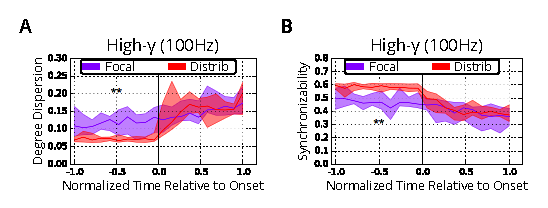
\includegraphics[width=\textwidth]{panel2.eps}
    \caption[Global synchronizability predicts seizure evolution]{\textbf{Differential pre-seizure synchronizability predicts seizure evolution.} (\textbf{A}) Heterogeneity, as measured by time-dependent dispersion of node strength in high-$\gamma$ functional networks, differed significantly in (i) partial seizures that remain focal ($N=19$), compared to (ii) partial seizures that generalize to surrounding tissue ($N=16$): (FDA, $p_\text{pre-seizure}=1.8\times10^{-4}$, $p_\text{seizure}=8.1\times10^{-1}$. (\textbf{B}) Time-dependent synchronizability in high-$\gamma$ functional networks differs significantly in the two types of seizures: (FDA, $p_\text{pre-seizure}=4.1\times10^{-4}$, $p_\text{seizure}=1.7\times10^{-1}$). Thick lines represent median, shaded area represents $1^{st}$ and $3^{rd}$ quartile. $P$-values are obtained via functional data analysis (FDA) where event labels (two seizure types) were permuted uniformly at random (see Methods): *$p<0.05$, **$p<0.001$. \label{ch5:fig2}}
\end{figure}


\subsection{Network Controllers of Synchronizability}
How might network heterogeneity regulate levels of synchronizability? Do a subset of nodes act as key controllers, or do all nodes contribute equally? To answer this question, we developed a novel method to assess the influence of a node on synchronizability. We define the \emph{control centrality} $c_i$ of node $i$ to be the fractional change in synchronizability following removal of node $i$ from the network (\textbf{Fig.~\ref{ch5:fig3}A}): $c_i=\frac{s_i-s}{s}$ where $s$ is the original synchronizability and $s_i$ is the synchronizability after node removal. The magnitude of $c_i$ can be interpreted as the overall strength of the node as a controller of synchronizability. If $c_i$ is positive, then synchronizability increases upon node removal, and the node is said to be a \emph{desynchronizing node}. If $c_i$ is negative, then synchronizability decreases upon node removal, and the node is said to be a \emph{synchronizing node}. As illustrated in \textbf{Fig.~\ref{ch5:fig3}A}, both desynchronizing and synchronizing network controllers are characteristic of heterogeneous networks, and tend to be located in the network periphery and network core, respectively.

\begin{figure}[H]
    \centering
    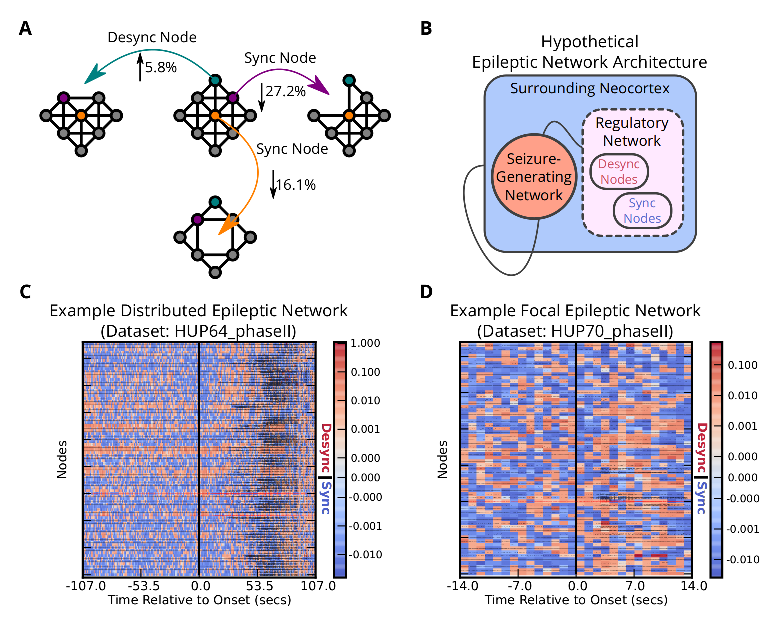
\includegraphics[width=\textwidth]{panel3.eps}
    \caption[Schematic of virtual cortical resection]{\textbf{Virtual cortical resection localizes network controllers.} (\textbf{A}) Effect of node removal on network synchronizability (control centrality) in a toy network. Highlighted node removals resulting in increased synchronizability (desynchronizing node; blue), decreased synchronizability (synchronizing nodes; purple and orange). The strongest desynchronizing node increased synchronizability by 5.8\% and was present in the network periphery, while the strongest synchronizing nodes decreased synchronizability by 27.2\% and 16.1\% and were located in the network core. (\textbf{B}) Hypothetical regulatory network employs desynchronizing and synchronizing nodes to regulate levels of synchronizability. (\textbf{C}) Control centrality in example distributed (and (\textbf{D}) focal) epileptic network events. ECoG signal is normalized by maximum amplitude. Red signals signify clinically-marked seizure-generating nodes. \label{ch5:fig3}}
\end{figure}

We used control centrality to assess the presence of desynchronizing and synchronizing controllers in the epileptic network, and to define their putative role in regulating synchronizability, a hallmark of seizure dynamics (\textbf{Fig.~\ref{ch5:fig3}B}). We observed that controller roles differed in their temporal dynamics, and in spatial distribution. In an example of a distributed epileptic network (see \textbf{Fig.~\ref{ch5:fig3}C}), we found clusters of desynchronizing nodes that switched to synchronizing nodes as the seizure began (and desynchronizing controllers appear elsewhere), and then switched back to desynchronizing nodes as the seizure terminated (and synchronizing controllers appear elsewhere). Interestingly, these coordinated dynamics occurred away from seizure-generating areas. In an example of a focal epileptic network (see \textbf{Fig.~\ref{ch5:fig3}D}), we observed less coordinated dynamics; preceding the seizure, desynchronizing and synchronizing controllers appeared dispersed across the network, while, after seizure-generation, more apparent clustering of desynchronizing and synchronizing nodes emerged away from the seizure-generating areas (see for example \textbf{Fig.~\ref{ch5:fig3}D}).

\subsection{Regulatory System Controls Seizure Dynamics}
Given that synchronizability appears to be driven by a small number of synchronizing and desynchronizing nodes in the tissue surrounding the seizure-generating area, we next asked whether these putative controllers displayed differential influence in different seizure types. To address this question, we separately computed the average of the control centrality over all time-windows in each epoch for the seizure-generating area and the surrounding tissue. In the seizure-generating area, we found no differences in the control centrality estimated during the pre-seizure epoch for the partial seizures that remained focal in comparison to the partial seizures that generalized to surrounding tissue. In contrast, in the surrounding tissue, we observed significantly greater control centrality in the focal in comparison to the generalized case (\textbf{Fig.~\ref{ch5:fig4}A}). No differences in control centrality were observed during the seizure epoch (\textbf{Fig.~\ref{ch5:fig4}B}). We interpret these findings as intuitively implying that controllers outside the seizure-generating area play an important role in constraining seizure evolution.

\begin{figure}[H]
    \centering
    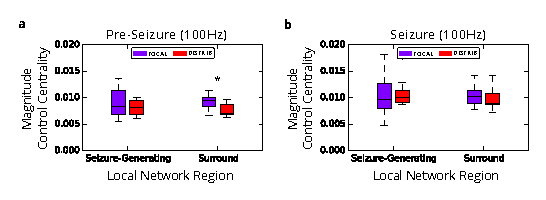
\includegraphics[width=\textwidth]{panel4.eps}
    \caption[Control centrality of surrounding network structures]{\textbf{Control centrality in surrounding network differentiates seizure type.} (\textbf{A}) Control centrality in the \textit{pre-seizure epoch} estimated within the seizure-generating area and within the surrounding tissue for partial seizures that remain focal ($N=19$) and that generalize to surrounding tissue ($N=16$): (rank-sum test; $p_\text{sz-gen}=6.8\times10^{-1}$, $p_\text{surround}=3.2\times10^{-3}$). Control centrality of the surrounding tissue is greater in the focal as opposed to the distributed epileptic networks. (\textbf{B}) Control centrality in the \textit{seizure epoch} estimated within the seizure-generating area and within the surrounding tissue for partial seizures that remain focal ($N=19$) and that generalize to surrounding tissue ($N=16$): (rank-sum test; $p_\text{sz-gen}=4.3\times10^{-1}$, $p_\text{surround}=2.4\times10^{-1}$); $p$-values are computed using a non-parametric Wilcoxon rank-sum test to account for uneven sample sizes across different seizure types. (\textbf{C}) Control centrality of desynchronizing nodes in the tissue surrounding the seizure generating area in both partial seizures that remain focal ($N=19$) and those that generalize to surrounding tissue ($N=16$): (FDA; $p_\text{pre-seizure}=9.2\times10^{-4}$, $p_\text{seizure}=2.9\times10^{-1}$). During the pre-seizure epoch, we observe significantly greater control centrality of desynchronizing nodes in partial seizures that remain focal \emph{versus} those that generalize to surrounding tissue. (\textbf{D}) Control centrality of synchronizing nodes in the tissue surrounding the seizure generating area in both partial seizures that remain focal ($N=19$) and those that generalize to surrounding tissue ($N=16$): (FDA; $p_\text{pre-seizure}=2.5\times10^{-2}$, $p_\text{seizure}=9.2\times10^{-1}$). During the pre-seizure epoch, we observe significantly greater control centrality of desynchronizing nodes in partial seizures that remain focal \emph{versus} those that generalize to surrounding tissue. \label{ch5:fig4}}
\end{figure}

Which type of putative control node (synchronizing or desynchronizing) plays a more prominent role in partial seizures that remain focal versus those that generalize to surrounding tissue? In pre-seizure epochs, we observed significantly stronger control centrality of both desynchronizing (\textbf{Fig.~\ref{ch5:fig4}C}) and synchronizing (\textbf{Fig.~\ref{ch5:fig4}D}) nodes in the focal compared to the distributed epileptic networks. Thus, both types of putative control nodes played a more prominent role in partial seizures that remained focal versus those that generalized to surrounding tissue. This suggests that focal epileptic networks exert a push-pull control mechanism to constrain seizure evolution. Note that this observation is specific to pre-seizure epochs: no differences were observed in synchronizing or desynchronizing control centrality during seizure epochs.

\section{Discussion}

In this work we asked, ``Is there a network-level control mechanism that regulates seizure evolution?'' To answer this question, we designed and applied a novel computational tool -- \emph{virtual cortical resection} -- to predict network response to removing regions in the epileptic network. Our work supports the notion that a regulatory system located outside the seizure-generating area consists of synchronizing and desynchronizing nodes, which constrain seizure evolution using an antagonistic, push-pull control mechanism.

\subsection{Spatial Extent of Seizure Evolution}
The spatial extent of the epileptic network driving seizure dynamics has been elusive. Epilepsy experts conventionally implicate the seizure-generating region as the underlying source of network dysfunction, and the surrounding irritative zone as a secondary site of abnormality that is not itself capable of independently generating seizures \cite{rosenow2001presurgical, nair2004critical}. Others have identified strong, tightly connected network hubs localized in areas outside the seizure-generating region that indicate a wider extent of network damage \cite{schevon2007cortical, zaveri2009localization-related, rummel2013systems-level}. Our results support the view that tissue surrounding the seizure-generating area displays abnormalities that support seizure evolution. Specifically, we observe the presence of putative control nodes within a broader heterogeneous network that may serve to discourage seizure spread by limiting synchronizability of healthy activity states. 

These findings may also have important neurobiological implications for epilepsy research. They raise questions such as, "What is the neuroanatomical substrate for network nodes that drive or contain seizures?" Might there be direct anatomical dysfunction such as loss of inhibiting inter-neurons, aberrant fiber-sprouting or changes in local gap junctions or ion channel expression that correlate with desynchronizing or synchronizing functional regions? Relating correlates of dysfunction from node resection and electrophysiologic studies to underlying neuroanatomy in applications of targeted drug-delivery remains a promising area of epilepsy research. 


\subsection{Push-Pull Control as a Regulatory Mechanism}
Controllability of functional brain networks is a burgeoning area of network neuroscience, particularly in the study of large-scale brain areas and the distributed circuits they constitute \cite{bassett2006adaptive, gu2014controllability}. However, these principles may have even greater impact in meso-scale brain networks, where local neural populations frequently switch between a wide variety of normal and abnormal rhythmic neural processes. Using virtual cortical resection, we observed the presence of specific nodes whose placement in the wider network suggests their critical role in controlling synchronization and desynchronization in seizure dynamics. These key areas display antithetical potential for controlling activity dynamics, and therefore we speculate that they may employ an antagonistic, push-pull control mechanism similar to that described in theoretical work in other systems \cite{he2014control}. Mechanistically, synchronizing controllers might pull the network towards a particular stable state, and, conversely, desynchronizing controllers might push the network away from the stable state. Such a mechanism also aligns with the recently proposed Epileptor model of seizure dynamics, where any brain network might be capable of seizure generation depending on its vulnerability to crossing a critical separatrix barrier \cite{jirsa2014nature, naze2015computational}. In the framework of the Epileptor, our results suggest that synchronizing and desynchronizing nodes might regulate a critical level of network stability and prevent the extent to which the network crosses a separatrix. 


\subsection{Methodological Limitations and Extensions}

An important clinical consideration related to this work is the sampling error inherent in any intracranial implantation procedure. Any of the techniques used to map epileptic brain usually yield incomplete representations of the epileptic network. It is not possible to fully record from the entirety of cortex in affected patients. In some cases this might mean that neither seizure onset zones nor all regions of seizure spread are fully delineated.

The virtual cortical resection approach can be extended to model other complex dynamics beyond independent node contributions to network synchronization. For example, we could iterate over all possible node resections to find the network configuration that optimizes synchronizability. Furthermore, in this work we apply virtual cortical resection to study a single topological metric, network synchronizability. Additional quantities of interest include measures of causal information flow \cite{korzeniewska2014ictal}.

\subsection{Clinical Impact}
Isolating the natural control mechanisms of brain function is critical for clinical translation. Enhancing and disrupting these natural control mechanisms could be a viable approach for introducing therapy with implantable devices for network disorders like epilepsy. Current methods of treating drug-resistant epilepsy rely on surgical resection or, more recently, implantable devices. However, predicting network response to therapy remains challenging. The virtual cortical resection technique is a novel, objective method of probing robustness and fragility upon removing components of the epileptic network. Using this method, we pinpointed putative network controllers that may be crucial for seizure evolution -- suggesting that resection of these regions may compromise key mechanisms to contain seizure activity.

This technique will require careful retrospective, and perhaps eventually prospective, trials to validate its utility. There are frequent examples of patients in whom seizures appear to be localized on intracranial EEG who go on to have recurrent or persistent seizures despite surgical resection or device placement. It is our hope that practical implementations of models like our virtual cortical resection may allow clinicians to predict response to therapy and provide a quantitative guide to what is now a process guided by manual interpretation of ECoG recordings. 

There may also be clinical implications beyond just guiding electrode placement for anti-epileptic devices. These studies might open the way towards more accurate electrophysiologically-guided cortical resection or perhaps pinpointed thermal ablation to specific network regions, similar to procedures done by cardiac electrophysiologists. These potential applications, while far off, offer considerable clinical advantage over the large cortical resections performed currently, with modest seizure-freedom rates.  

\section{Methods}
\subsection{Patient Data Sets}
\subsubsection{Ethics Statement}
All patients included in this study gave written informed consent in accordance with the Institutional Review Board of the University of Pennsylvania.

\subsubsection{Electrophysiology Recordings}
Ten patients undergoing surgical treatment for medically refractory epilepsy believed to be of neocortical origin underwent implantation of subdural electrodes to localize the seizure onset zone after presurgical evaluation with scalp EEG recording of ictal epochs, MRI, PET and neuropsychological testing suggested that focal cortical resection may be a therapeutic option. Patients were then deemed candidates for implantation of intracranial electrodes to better define epileptic networks. De-identified patient data was retrieved from the online International Epilepsy Electrophysiology Portal (IEEG Portal) \cite{wagenaar2013multimodal}.

ECoG signals were recorded and digitized at 500 Hz sampling rate using Nicolet C64 amplifiers and pre-processed to eliminate line noise. Cortical surface electrode (Ad Tech Medical Instruments, Racine, WI) configurations, determined by a multidisciplinary team of neurologists and neurosurgeons, consisted of linear and two-dimensional arrays (2.3 mm diameter with 10 mm inter-contact spacing) and sampled the neocortex for epileptic foci (depth electrodes were first verified as being outside the seizure onset zone and subsequently discarded from this analysis). Signals were recorded using a referential montage with the reference electrode, chosen by the clinical team, distant to the site of seizure onset and spanned the duration of a patient's stay in the epilepsy monitoring unit. See Table 1 for demographic and clinical information.

\begin{table}[H]
    \scriptsize
    \centering
    \begin{tabular}{|x{2cm}|x{0.5cm}|x{0.75cm}|x{2cm}|x{1.5cm}|x{1.25cm}|x{1cm}|x{1cm}|x{1.40cm}|}
        \hline
        Patient\newline (IEEG Portal) & Sex & Age & Seizure Onset & Etiology & Seizure Type (N) & Imaging & Outcome \\ \hline \hline
        \verb|HUP64_phaseII| & M & 03/20 & Left frontal & Dysplasia & CP+GTC (1) & L & I\\ \hline
        \verb|HUP65_phaseII| & M & 02/36 & Right temporal & Auditory reflex & CP+GTC (3) & N/A & I\\ \hline
        \verb|HUP68_phaseII| & F & 15/26 & Right temporal & Meningitis & CP (1), CP+GTC (4) & NL & I\\ \hline
        \verb|HUP70_phaseII| & M & 10/32 & Left perirolandic & Cryptogenic & SP (8) & L & NR\\ \hline
        \verb|HUP72_phaseII| & F & 11/27 & Bilateral left & Mesial temporal sclerosis & CP+GTC (1) & L & NR\\ \hline
        \verb|HUP73_phaseII| & M & 11/39 & Anterior right frontal & Meningitis & CP+GTC (5) & NL & I\\ \hline
        \verb|HUP78_phaseII| & M & 00/54 & Anterior left temporal & Traumatic injury & CP (5) & L & III\\ \hline
        \verb|HUP79_phaseII| & F & 11/39 & Occipital & Meningitis & CP (3) & L & NR\\ \hline
        \verb|HUP86_phaseII| & F & 18/25 & Left temporal & Cryptogenic & CP+GTC (2) & NL & II\\ \hline
        \verb|HUP87_phaseII| & M & 21/24 & Frontal & Meningitis & CP (2) & L & I\\ \hline
    \end{tabular}
    \caption[Patient data set for Chapter \ref{ch:selfreg}]{\textbf{Patient information.} Patient data sets accessed through IEEG Portal (http://www.ieeg.org). Age at first reported onset and at phase II monitoring. Localization of seizure onset and etiology is clinically-determined through medical history, imaging, and long-term invasive monitoring. Seizure types are SP (simple-partial), CP (complex-partial), CP+GTC (complex-partial with secondary generalization). Counted seizures were recorded in the epilepsy monitoring unit. Clinical imaging analysis concludes L, Lesion; NL, non-lesion. Surgical outcome was based on Engel score (scale: I-IV, seizure freedom to no improvement; NR, no-resection; NF, no follow-up). M, male; F, female. \label{ch5:tab1}}
\end{table}

\subsubsection{Description of Epileptic Events}
We analyzed 19 partial seizures (simple and complex) and 16 partial seizures that generalized to surrounding tissue, forming a population of focal and distributed epileptic networks, respectively. Seizure type, onset time, and onset localization were marked as a part of routine clinical workup.

The seizure state spanned the period between clinically-marked earliest electrographic change (EEC) \cite{litt2001epileptic} and termination; and the pre-seizure state spanned a period equal in duration to the seizure state and ended immediately prior to the EEC (we refer to each pair of pre-seizure and seizure states as an \textit{event}).

\subsection{Functional Network Construction}
\subsubsection{Pre-Processing}
ECoG signals from each event were divided into 1-second, non-overlapping, wide-sense stationary time-windows in accord with related studies \cite{kramer2010coalescence}. In each time window, signals were re-referenced to the common average reference \cite{kramer2010coalescence, towle1999electrocorticographic} to account for variation in reference location across patients and to avoid broad field effects that may bias connectivity measurements erroneously in the positive direction.

\subsubsection{Coherence Estimation}
We constructed functional networks in each time-window using multitaper coherence estimation, which defines a network connection between electrode pairs as the power spectral similarity of signal activity over a specific frequency band. We applied the \textit{mtspec} Python implementation \cite{prieto2009fortran} of multitaper coherence estimation with time-bandwidth product of 5 and 8 tapers in accord with related studies \cite{kramer2011emergence}. Based on vast literature implicating high-frequency oscillations and $\gamma$ activity as drivers of epileptic activity, we primarily studied functional connectivity in the high-$\gamma$ band (95--105 Hz). This frequency range represents relatively local neural population dynamics that are largely unaffected by volume conduction.

\subsection{Metrics of the Time-Varying Functional Network}

\subsubsection{Network Geometry}
In our network analysis, we refer to heterogeneity of network architecture in the context of node strength, also known as weighted degree. We measure a time-varying quantity of heterogeneity: the dispersion of the degree distribution in each time window. We use a non-parametric, interquartile distance measure to quantify dispersion. The interquartile distance is the 75th percentile subtracted by the 25th percentile of a distribution.

\subsubsection{Network Synchronizability}
A recent trend in studying functional networks is to model dynamic geometric structure that evolves through states \cite{wulsin2013parsing, rummel2013systems-level, burns2014network}. Building on the classical notion of stability of the synchronized state in static networks, we fit a popular synchronizability model for dynamic networks \cite{gomez2013diffusion} to account for time-varying structure of the functional networks in our study. As a simplification for our analysis, we assume functional networks between time-windows are independent.

To quantify synchronizability, we first estimated the time-varying Laplacian matrix $\textbf{L}(t)$ for each time-window $t$ of the functional network. Intuitively, each entry $l_{ij}(t)$ of $\textbf{L}(t)$ quantifies how easily information could diffuse between nodes $i$ and $j$ based on the relative connectivities of both nodes to all other nodes in the network. Next, we computed the eigenspectrum of $\textbf{L}(t)$ and calculated the ratio of the second-smallest eigenvalue $\lambda_2$ to the largest eigenvalue $\lambda_\text{max}$ for each $t$, resulting in network synchronizability $s_{t}=\frac{\lambda_2}{\lambda_\text{max}}$ (larger values of $s(t)$ correspond to greater state stability) \cite{barahona2002synchronization}. The \textbf{Supplementary Note} provides details of the \textit{master stability function} formalism behind synchronizability and its relationship to state stability. 

\subsubsection{Virtual Cortical Resection}
To model potential effects of resecting or lesioning regions of brain networks, we develop a virtual cortical resection technique. Generally, the approach allows us to ask how network topology might change upon removing one or more nodes or connections in the network. In time-varying networks, virtual cortical resections may be useful in patterned lesioning schemes for implantable devices that continuously modulate brain state away from seizures \cite{stanslaski2012design, afshar2013translational}.

Here, we tailored virtual cortical resection to study putative controllers that regulate synchronizability in the epileptic network. We measure the control centrality, the contribution of a node to network synchronizability, by applying virtual cortical resection to each node in each time-window of the functional network. The control centrality identifies a node as a desynchronizing ($c_i > 0$) or synchronizing ($c_i < 0$) controller. The \textbf{Supplementary Material} explores the relationship between control centrality and other topological properties of networks.

\subsubsection{Statistical analysis}
We compared time-varying network metrics between partial seizures that remain focal and partial seizures that generalize to surrounding tissue. We performed this comparison by (i) normalizing each seizure event into 20 sequential time-bins spanning the pre-seizure and seizure states and (ii) employing functional curve analysis to statistically test differences in temporal dynamics between seizure type, independently in each state. We assigned $p$-values to each state by re-assigning events uniformly at random to seizure types up to 1,000,000 times and computing the mean area between the resulting functional curves.

\section{Acknowledgments}
AK and BL acknowledge support from the National Institutes of Health through awards \#R01-NS063039, \#1U24 NS 63930-01A1, the Citizens United for Research in Epilepsy (CURE) through Julie's Hope Award, and the Mirowski Foundation. DSB acknowledges support from the John D. and Catherine T. MacArthur Foundation, the Alfred P. Sloan Foundation, the Army Research Laboratory, the Institute for Translational Medicine and Therapeautics, the National Institute of Mental Health through award number 2-R01-DC-009209-11 (Thompson-Schill), and the National Science Foundation awards CRCNS BCS-1441502 and BCS-1430087 through the ENG, CISE, and SBE directorates. The content is solely the responsibility of the authors and does not necessarily represent the official views of any of the funding agencies.

\section{Supplemental Information}
\subsection{Master Stability Function for Network Synchronizability}
The traditional notion of connectivity in brain networks is the statistical relationships between cortical regions and how such relationships change with time \cite{friston2011functional, hutchison2013dynamic}. In addition to describing topology, connectivity can be used to query how neural processes at each node diffuse along pathways between cortical areas. The latter study of network organization asks the nature of diffusive dynamics on static or time-varying networks. 

Modeling diffusion of processes over the network is critical for asking pertinent questions in neuroscience more generally and epilepsy more specifically, such as "How does brain activity synchronize during seizures?" As functional brain networks re-organize, the ability for neural processes at each node to synchronize also changes, a property known as \textit{synchronizability} \cite{barahona2002synchronization}. These attributes are captured by a generative model for diffusion over the networks, called the \textit{master stability function} \cite{pecora1998master, gomez2013diffusion} -- defined as:
\begin{equation}\label{masterstab}
    \dot{x_i}(t) = f(x_i(t)) + \sigma(t)\sum\limits_{j=1}^{N}A_{ij}(t)(x_j(t) - x_i(t))
\end{equation}
where $x_i(t)$ represents the dynamical state of node $i$, $f$ is a function describing independent node dynamics, $\sigma$ is a diffusion constant, $A(t)$ is an $N \times N$ adjacency matrix of connection weights between $N$ network nodes. For a time-varying functional network, where each time window is assumed independent, the solution of Eqn. (\ref{masterstab}) is given by:
\begin{equation}\label{lapl}
    \dot{x}(t) = -\mathcal{L}(t)x(t)
\end{equation}
where $\mathcal{L}$ is the graph Laplacian whose entries $l_{ij}$ quantify how easily neural processes can diffuse between nodes $i$ and $j$. For a given network configuration, the potential for dynamics at each node to achieve equivalence around a state $q(t)$ such that $q(t)=x_1(t)=x_2(t)=...=x_N(t)$ is the network synchronizability $s(t)$. The stability of the synchronized state $q(t)$ is quantified by the eigenvalues of $\mathcal{L}$ such that:
\begin{equation}\label{sync}
    s(t) = \frac{\lambda_2}{\lambda_\text{max}}
\end{equation}
where $\lambda_2$ and $\lambda_\text{max}$ are the second-smallest and largest eigenvalues, respectively. Larger values of $s(t)$ correspond to greater potential for the network to stably synchronize.   

\subsection{Virtual Cortical Resection}
In the previous subsection we explored methods to query how easily diffusion dynamics on a network can synchronize. Synchronizability is governed by network organization, and as the network reconfigures over time so does its potential to synchronize. In this work we ask a non-trivial question regarding network synchronizability, "Which nodes are most important controllers for regulating synchronizability?" Answering this question may have significant impact in understanding which regions of the network naturally maintain stability in the synchronized state.

Our approach was to independently remove network regions (virtual cortical resection) and measure change in the ability of the modified network to stably synchronize. The removed region was assigned a control centrality equal to the fractional change in synchronizability in the modified network from the original network. Based on the relative increase or decrease of synchronizability, we found that individual nodes can assist in stabilizing the synchronized state by either desynchronizing or synchronizing the network. 

Importantly, we investigated whether control centrality is an emergent property of network topology or simply related to the average strength of connections from that node. To this end, we computed the amount of variance in control centrality that is explained by nodal strength during the pre-seizure and seizure epochs in the example focal (\textbf{Fig.~\ref{ch5:figS1}A}) and distributed epileptic networks (\textbf{Fig.~\ref{ch5:figS1}B}). In both events we observed low linear relationships between control centrality and degree centrality in the pre-seizure and seizure epochs. These results suggest control centrality is a novel measure of network geometry specifically related to the synchronization of dynamic processes.   

\begin{figure}[H]
    \centering
    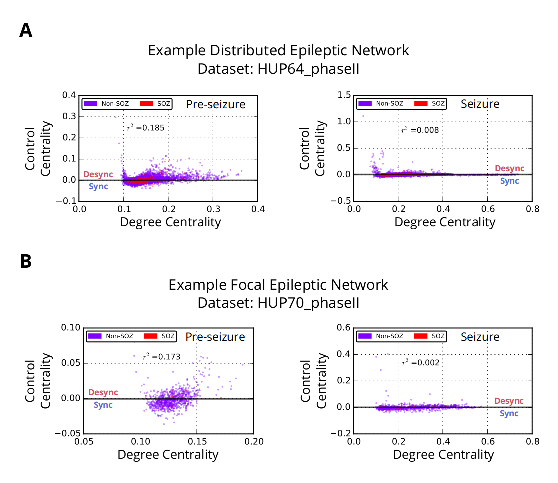
\includegraphics[width=\textwidth]{panelS1.eps}
    \caption[Control centrality as a network measure]{\textbf{Control centrality as a network measure.} (\textbf{A}) Relationship between control centrality and weighted degree centrality over all time-windows during pre-seizure (\textit{left}) and seizure (\textit{right}) epochs in a sample event from the \textit{distributed epileptic network}. (\textbf{B}) Relationship between control centrality and weighted degree centrality over all time-windows during pre-seizure (\textit{left}) and seizure (\textit{right}) epochs in a sample event from the \textit{focal epileptic network}. $r^2$ measures the amount of variance in control centrality explained by weighted degree centrality. \label{ch5:figS1}}
\end{figure}
